% \section{Development}
% \label{sec:development}

% This section presents the operation of the application and the measurement tools used in the tests.

\subsection{Photo Application}
Two photo gallery applications were developed: one focused on server-side rendering, and the other on client-side rendering, along with a selection page where the user can choose which rendering method will be displayed. Both applications were built using the same HTML structure, the same CSS styles, and without inserting any scripts, in order to prevent side effects on test results. Figure~\ref{fig:jsonStructure1} shows the initial selection page, while Figure~\ref{fig:jsonStructure2} shows the application running with client-side rendering using the smallest data size.

% \begin{figure}[h]
% \centering
% \begin{minipage}{0.47\textwidth}
%     \centering
%     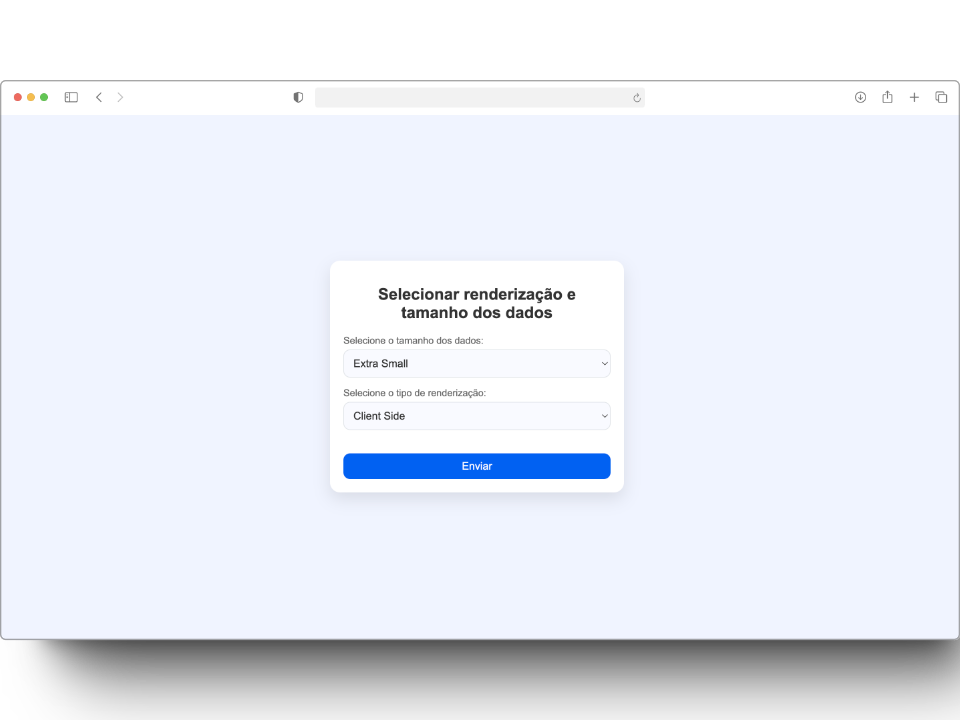
\includegraphics[width=\textwidth]{img/app02.png}
%     \caption{Data size and rendering type selection}
%     \label{fig:jsonStructure1}
% \end{minipage}\hfill
% \begin{minipage}{0.47\textwidth}
%     \centering
%     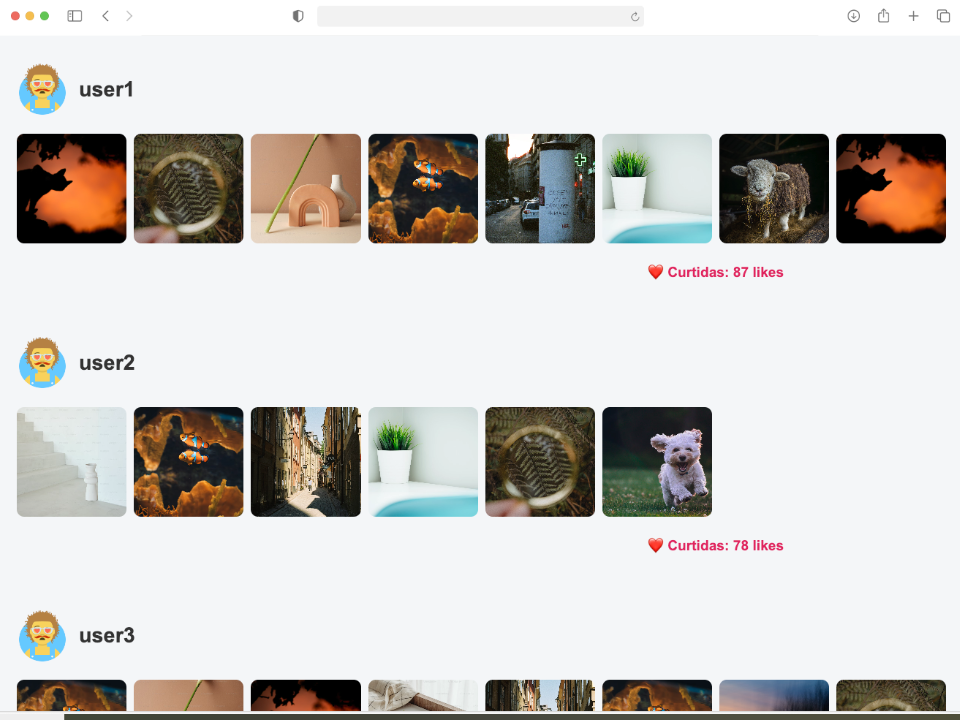
\includegraphics[width=\textwidth]{img/app-client.png}
%     \caption{Application using extra small data and CSR rendering}
%     \label{fig:jsonStructure2}
% \end{minipage}
% \end{figure}




\begin{figure}[h]
\centering
    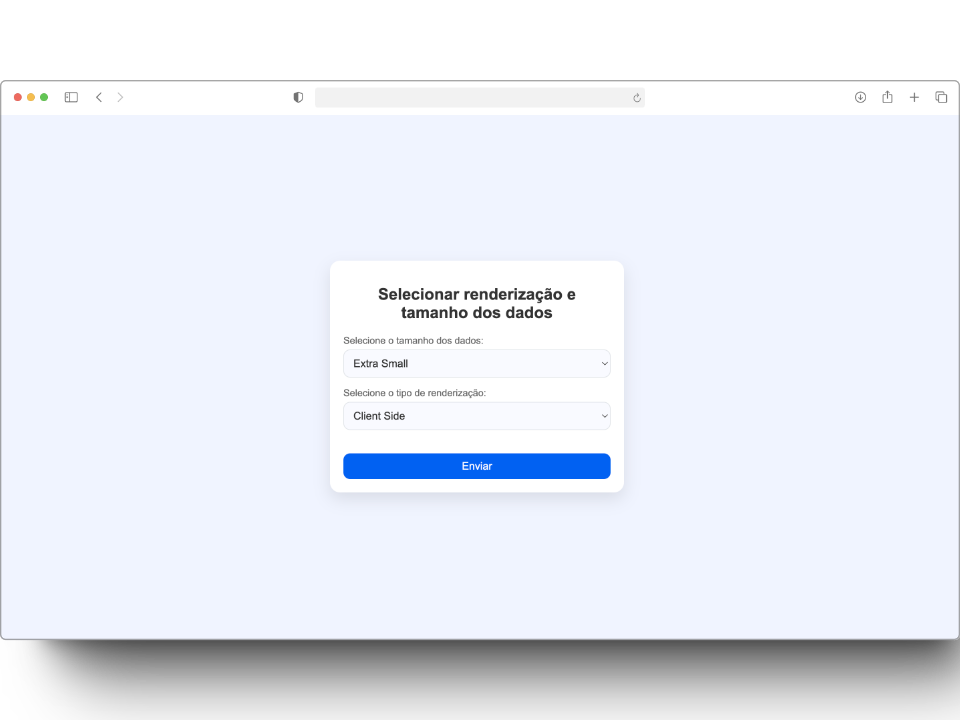
\includegraphics[width=.45\textwidth]{img/app02.png}
    \caption{Data size and rendering type selection}
    \label{fig:jsonStructure1}
\end{figure}

\begin{figure}[h]
\centering
    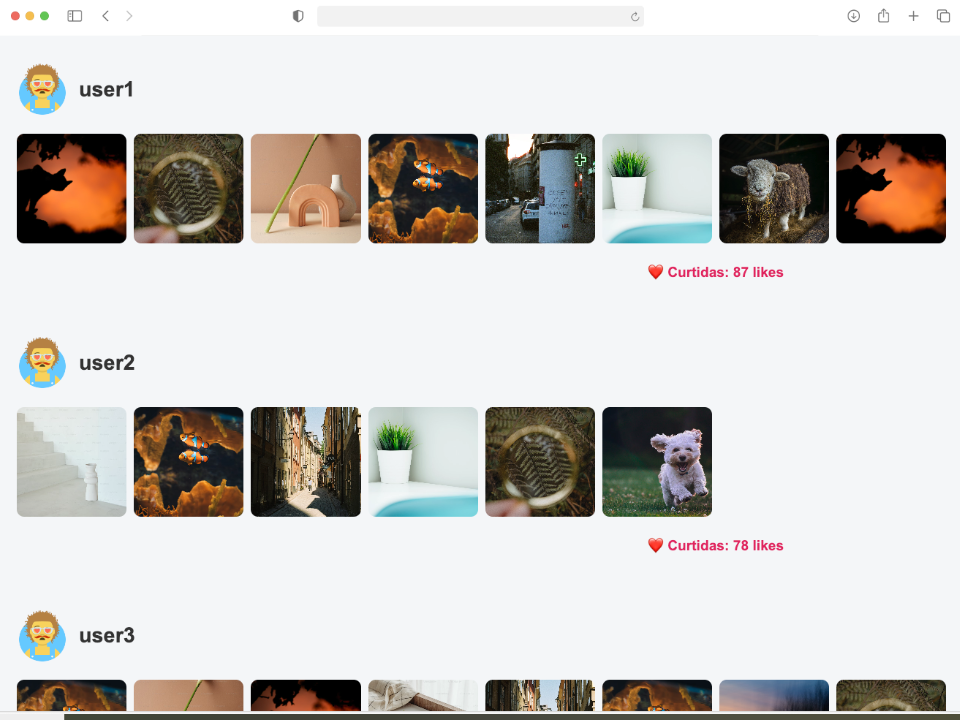
\includegraphics[width=.45\textwidth]{img/app-client.png}
    \caption{Application using extra small data and CSR}
    \label{fig:jsonStructure2}
\end{figure}